\documentclass[12pt, oneside, a4paper]{mwbk}
\usepackage[UTF8]{inputenc}
\usepackage[polish]{babel}
\usepackage[OT4]{fontenc}

\usepackage{graphicx}
\usepackage{verbatim}
\usepackage{amsfonts}

\usepackage{enumitem}
\usepackage[noend]{algorithmic}
\usepackage[ruled]{algorithm}

\usepackage{color}
\usepackage[normalem]{ulem}

\usepackage{rotating}
\usepackage{float}
\usepackage{textpos}

\linespread{1,3}
\oddsidemargin = 10pt
\textwidth = 470pt

\hyphenpenalty=1000
\tolerance=500

\begin{document}
\author{Łukasz Kowalczyk}
\title{Technologia OpenCL w symulacji bryły sztywnej}
\begin{titlepage}
\thispagestyle{empty}
\begin{textblock}{1}(-2.65,-1.65)

\includegraphics{figures/tytulowa_pusta_mgrinz.pdf}
\end{textblock}
\vspace{7.3cm}
\begin{center}
\fontfamily{ptm}
\selectfont
\Huge
Technologia OpenCL w symulacji \\
dynamiki bryły sztywnej
\end{center}
\begin{center}
\fontfamily{ptm}
\selectfont
Praca dyplomowa inżynierska
\end{center}
\vspace{7.9cm}
\begin{center}
\fontfamily{ptm}
\selectfont
\hspace{-1cm}
\begin{tabular}{l}
Wydziaż Fizyki Technicznej, Informatyki i Matematyki Stosowanej \\
Promotor: dr inż. Dominik Szajerman \\
Dyplomant: Łukasz Kowalczyk \\
Nr albumu: 157889
\end{tabular}
\end{center}
\vspace{-.5cm}
\begin{center}
\fontfamily{ptm}
\selectfont
\begin{textblock}{13}(0,0.4)
Łódź, 2014
\end{textblock}
\end{center}
\end{titlepage}

\tableofcontents

\chapter{Wprowadzenie}
\label{t:int}

\section{Wstęp}
Początki obliczeń z wykorzystaniem akceleracji układów GPU związane są z przetwarzaniem potokowym oraz obliczeniami równoległymi. Jedne z pierwszych superkomputerów umożliwiały zdecydowanie zwiększoną wydajność dla zadań, które były podzielone na operacje powtarzalne. Pierwszy układ GPU został wprowadzony na rynek dzięki firmie Nvidia w 1999 roku \cite{nvidia}. Wtedy też rozpoczętko wykorzystywać te układy do obliczeń ogólnego przeznaczenia. \\
W roku 2001, wraz z wprowadzeniem programowalnego potoku renderingu oraz wsparcia dla obliczeń liczb zmiennoprzecinkowych, zaczęto wykorzystywać układy GPU do obliczeń niezwiązanych z grafiką. Pierwsze wersje shaderów były dość ograniczone ( np. dla Vertex Shadera 1.1 możliwe było użycie jedynie 128 instrukcji). Kolejne wersje znacznie zwiększały swoje możliwości ( 512 instrukcji dla Shader Model 3.0 oraz do 64 000 instrukcji dla Shader Model w wersji 4.0) \cite{wiki1}. \\
Zainteresowanie możliwościami obliczeniowymi kolejnych układów było duże, dlatego też w listopadzie 2006 roku Nvidia opracowała technologię CUDA. Pozwala ona na wykorzystanie mocy obliczeniowej procesorów GPU do rozwiązywania problemów numerycznych zdecydowanie wydajniej, niż wykonałby je procesor ogólnego zastosowania. Niestety tachnologia ta może być wykorzystana jedynie z kartami firmy Nvidia. W 2009 roku opracowany został przez firmę Apple Inc. otwarty framework OpenCL, który podobnie jak CUDA pozwala wykorzystać procesory graficzne do wykonania obliczeń, jednak w przeciwieństwie do technologii firmy Nvidia, OpenCL współpracuje z układami graficznymi wszystkich wiodących producentów a ponadto umożliwia uruchomienie zapisanych w nim kerneli na procesorach ogólnego przeznaczenia. \\
Wykorzystanie układów GPU znalazło zastosowanie w wielu dziedzinach, zaczynając od wsparcia naukowców przy tworzeniu nowych leków, poprzez obliczanie symulacji ruchu ciał niebieskich, przyspieszenia obliczeń związanych z kryptografią, aż po wykorzystanie w grach komputerowych do obliczań zwiazanych z fizyką (symulacje zachowań cieczy, efekty cząsteczkowe czy też wsparcie w obliczaniu kolizji).

\section{Cel}
Celem pracy jest stworzenie symulacji bryły sztywnej wykorzystując otwarty framework OpenCL do akceleracji obliczeń, a zatem do przemieszczania obiektów, znajdowania kolizji z innymi obiektami oraz reagowania na zderzenia. Praca zakłada również implementację komunikacji części bazowej programu z układem GPU oraz implementację uproszczonego wyświetlenia symulowanych brył przy użyciu technologii OpenGL.

\section{Założenia}
Praca zakłada wykorzystanie technologii OpenCL w wersji 1.2 do wykonania obliczeń fizycznych. Użycie technologii OpenGL w wersji 3.1 do wyświetlania efektów działania aplikacji zostanie wsparte dodatkową biblioteką glfw w wersji 3 \cite{GLFW}. Część bazowa programu umożliwiająca wykorzystanie OpenCL oraz OpenGL została napisana w języku C++. Do tworzenia samego projektu posłużyło środowisko IDE QTCreator 1.8.4 a do zarządzenia procesem kompilacji narzędzie Cmake w wersji 2.8. \\
Symulacja brył odbywa się w przestrzeni posiadającej grawitację ziemską przybliżoną do wartości 9.81 $m \over s_2$ oraz podłoże posiadające wagę zbliżoną do nieskończoności (m = $\infty$), na które nie działa siła grawitacji.

\section{Zakres pracy}
Pierwszy rozdział pracy dotoczy technologii OpenCL. Zostanie w nim omówiona architektura oraz ogólna zasada działania. Przedstawiony zostanie również sprzęt użyty do tworzonego oprogramowania.\\
Kolejny rozdział dotyczy technologii OpenGL. Przedstawione zostaną wstępne informacje o tej technologii, przedstawiony rozwój wraz z nowymi jej wersjami oraz omówione wykorzystanie technologii w projekcie.\\
Następny rozdział zawiera omówienie algorytmu sprawdzającego kolizję. Omówiony zostanie algorytm sprawdzania zderzeń między obiektami symulacji, zastosowane rozszerzenie podstawowej wersji algorytmu oraz problemy, które towarzyszą wykorzystaniu tej metody testowania kolizji.\\
Ostatni rozdział przedstawia konkretne zastosowanie technologii OpenCL przy obliczeniach związanych z symulacją. % Wstęp
\chapter{OpenCL}

\section{Wprowadzenie}
OpenCL (Open Computing Language) jest standardem tworzenia oprogramowania stworzonym przez Khronos Group, który powstał w celu wsparcia w tworzeniu oprogramowania z wykorzystaniem mocy zarówno współczesnych kart graficznych (GPU) jak i procesorów (CPU). Jedną z głównych zalet OpenCL jest otwartość standardu, co umożliwia wykorzystanie technologii opierając się o sprzęt wielu producentów ( np. Nvidia, Amd, Intel).

\section{Składniki środowiska OpenCL}
Idea funkcjonowania platformy OpenCL została przedstawiona na rysunku 2.1. \\
\begin{figure}[h]
\centering
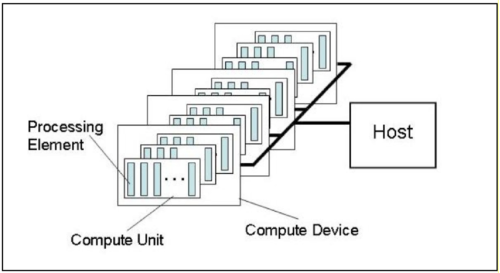
\includegraphics[width=0.8\textwidth]{figures/opencl_platform_model.png}
\caption{Model platformy OpenCL.}%
\label{rys:OpenCL Platform Model}
\end{figure}
Środowisko składa się z hosta – „gospodarza”, nakazujacego wykonanie konkretnego ciagu instrukcji urządzeniom obliczeniowym (Compute Device). Każde urządzenie posiada własny zestaw jednostek przetwarzających, na których istrukcje są wykonywane.

\section{Architektura CL}
Architektura OpenCL składa się z trzech zasadniczych części: specyfikacji języka, API platformy i API czasu wykonania. Specyfikacja języka OpenCL definiuje składnię programów i kerneli,które oparte są na zmodyfikowanym standardzie ISO C99, zawierającym część dodanych, zmienionych oraz usuniętych słów kluczowych. Cześć funkcjonalności również została usunięta z specyfikacji językowej, gdyż zostały one przeniesione do pozostałych dwóch części architektury. \\
API platformy umożliwia hostowi uruchamianie stworzonych kerneli na urządzeniach obliczeniowych. Realizuje ono również koncepcję kontekstu. Kontekst jest kontenerem grupującym urządzenie z przeznaczoną dla niego zawartością pamięci oraz kolejkami zadań. Przy pomocy API platformy realizowane jest przekazywanie danych między hostem a urządzeniem obliczeniowym. \\
API czasu wykonania wykorzystuje dostarczone przez platformę konteksty do kontrolowania kompatybilnych urządzeń. Przy jego pomocy odbywa się zarządzanie kolejkami zadań, obiektami pamięci i kernelami. Za poś rednictwem API czasu wykonania odbywa się również kolejkowanie kerneli na konkretnych urządzeniach.

\section{Paralelizm danych}
OpenCL, podobnie jak karty graficzne, które są główną grupą urządzeń wykorzystujących tą technologię, działa na zasadzie paralelizmu danych. W przeciwieństwie do paralelizmu zadań, który zakłada wykonanie różnych ciągów instrukcji w tym samym czasie, OpenCL zakłada wielokrotne wykonanie identycznego zadania wykorzystując jednak inne zestawy danych. \\
Paralelizm danych jest tutaj zrealizowany za pośrednictwem programów, które składają się z jednego lub więcej kerneli. Program poza samym kernelem może też zawierać dodatkowo dane stałe oraz funkcje, z których korzystają kernele. Podczas wykonania kernela przedstawione w nim zadanie wykonywane jest równolegle na elementach przetwarzających urządzenia obliczeniowego, tzw. work-itemy. \\

\section{Grupy robocze oraz zadania}
Jak przedstawiono na rysunku 2.2, ciągi instrukcji powiązane są ze sobą w grupy robocze. \\
\begin{figure}[h]
\centering
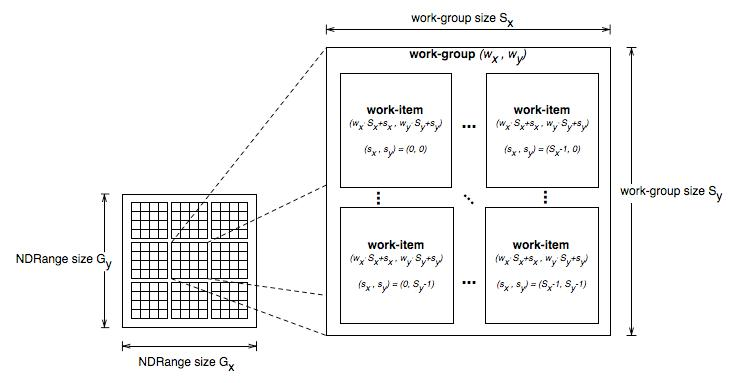
\includegraphics[width=0.8\textwidth]{figures/ndrange.jpg}
\caption{OpenCL NDRange.}%
\label{rys:ndrange}
\end{figure}
Obszar NDRange jest metodą słuzącą do organizacji pamięci i zaplanowania zadań w architekturze OpenCL. NDRange to jedno, dwu lub trzy wymiarowa przestrzeń. Jest ona podzielona na grupy robocze. Każda grupa posiada swój indeks, po którym można określić jej pozycję w przestrzeni. Każdy ciąg instrukcji, stanowiący odrębne zadanie kernela , dysponuje unikalnym globalnym numerem identyfikacyjnym a także unikalnym lokalnym numerem identyfikacyjnym wewnątrz każdej z grup.  \\
Tak podzielona przestrzeń wynika z architektury OpenCL. Dzięki identyfikatorom można skorzystać z bariery lokalnej, czyli ograniczyć synchronizację wątków działających tylko w ramach grupy roboczej.

\section{Zarządzanie pamięcią w OpenCL}
W OpenCL wyszczególnione są cztery przestrzenie pamięci. Są nimi:
\begin{itemize}
  \item Pamięć globalna - wszystkie wątki w grupach roboczych posiadają pełen dostęp (zapis i odczyt) do pamięci. Jest największym dostępnym obszarem pamięci jednak oferuje najwolniejszy dostęp
  \item Pamięć prywatna - dostęp do pamięci jedynie dla zadania, które zaalokowało pamięć podczas wykonywania danej instancji kernela.
  \item Pamięć lokalna - wszystkie wątki w danej grupie roboczej posiadają pełen dostęp do pamięci, jednak jest ona nieosiągalna dla wątków z innych grup. Możliwe jest zmapowanie obszaru pamięci na pamięć lokalną w celu uzyskania przyspieszonego czasu dosępu, jednak nie jest to wspierane przez wszsytkie urządzenia.
  \item Pamięć stała. W tej kategorii pamięci przechowywane są stałe wartości podczas wykonania całej operacji kernela. Jest ona inicjalizowana przez hosta.
\end{itemize}

\section{Urządzenia wykorzystane do testów}
\subsection{NVIDIA GTX 760}
Do testów została wykorzystana karta NVIDIA GeForce GTX 760, przedstawiona na rysunku 2.3. \\
\begin{figure}[h]
\centering
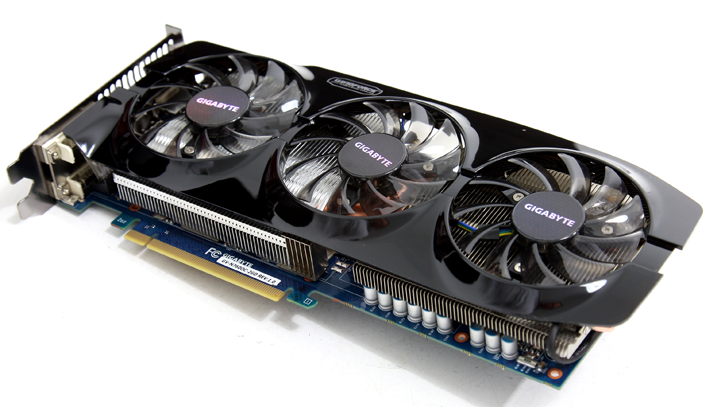
\includegraphics[width=0.8\textwidth]{figures/gtx.png}
\caption{NVIDIA GeForce GTX 760.}%
\label{rys:NVIDIA GeForce GTX 760}
\end{figure}
Karta została wyposażona w 1152 rdzeni CUDA (OpenCL uznaje je jako elementy przetwarzające) zebranych w 32 jednostkach obliczeniowych. Każdy z rdzeni jest taktowany zegarem o częstotliwości 1085 MHz. Maksymalna wydajność karty podczas obliczeń podwójnej precyzji wynosi 94 GFLOPsów (tysięcy operacji zmiennoprzecinkowych na sekundę), zaś podczas obliczeń w pojedynczej precyzji 2258 GFLOPSów. Karta została wyposażona w 2GB pamięci RAM typu GDDR5, taktowanej efektywną prędkością 1502 MHz. Wspiera standard OpenCL w wersji 1.2 oraz 2.0.\\
\newpage
\subsection{Intel\textregistered Core\texttrademark i5-3570K}
Do testów został wykorzystany również procesor Intel\textregistered Core\texttrademark i5 model 3570K przedstawiony na rysunku 2.4. 
\begin{figure}[h]
\centering
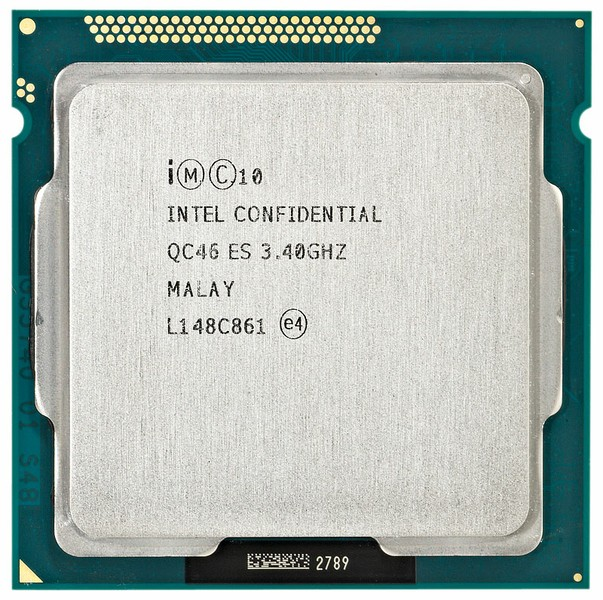
\includegraphics[width=0.3\textwidth]{figures/intel.jpg}
\caption{Intel\textregistered Core\texttrademark i5-3570K.}%
\label{rys:Intel Core i5-3570K}
\end{figure}
\\Posiada cztery rdzenie, które mogą na raz przetwarzać maksymalnie do czterech wątków. Procesor pracuje w zakresie częstotliwości 3.4 - 3.8 GHz. Jest to urządzenie zrealizowane w technologii 22nm o archtekturze noszącej nazwę Ivy Bridge. Posiada on 128 KB pamięci L1 Data Cache oraz 128 KB L1 Instruction Cache. Urządzenie to wspiera standard OpenCL w wersji 1.2.
 %OpenCL
\chapter{Porównanie czasu wykonywanych obliczeń przy użyciu GPU oraz CPU}

\section{Podsumowanie}

\section{Wnioski} %openGL
\chapter{Dynamika bryły sztywnej}
\section{Bryła sztywna}
Bryła sztywna inaczej ciało sztywne jest to obiekt, w którym poszczególne punkty (np.~cząsteczki) pozostają w stałych odległościach od siebie. Ciało sztywne nie zmienia swojego kształtu oraz posiada stałą gęstość.\\
Opisując dynamikę bryły sztywnej należy zwrócić uwagę na dwa rodzaje ruchu.
\subsection{Ruch postępowy}
Każdy odcinek łączący dwa dowolne punkty ciała bryły będzie równoległy do odcinka łączącego te same dwa punkty, ale w poprzednim położeniu. Wszystkie punkty bryły poruszają się w danym momencie z jednakową prędkością liniową a podczas ruchu jednostajnie zmiennego będą miały również takie samo przyspieszenie. Dlatego też ruch postępowy dla~bryły sztywnej jest identyczny jak dla ruchu punktu materialnego
\subsection{Ruch obrotowy}
Wszystkie punkty bryły sztywnej, za wyjątkiem tych leżących na osi obrotu, poruszają się po okręgach o promieniu równym \verb$r$, równych odległości punktów od osi obrotu. Prędkość kątowa bryły będzie wynosić\begin{equation}\omega=\frac{v_i}{r_i}\end{equation}
gdzie \verb$v$ to prędkość liniowa. Zatem energię kinetyczną ciała można obliczyć z zależności:
\begin{equation}E_i=\frac{1}{2}mr_i^2\omega_i^2\end{equation}
Całkowita energia kinetyczna bryły w tym ruchu jest równa sumie energii kinetycznych jej poszczególnych punktów. Z definicji bryły sztywnej wynika, że w tym ruchu wszystkie punkty będą miały taka samą prędkość kątową. Tak więc całkowitą energię kinetyczną bryły można przedstawić w postaci wzoru:
\begin{equation}E_c=\frac{1}{2}(\sum_i^nm_ir_i^2)\omega^2\end{equation}
Iloczyny \begin{equation}m_i r_i\end{equation} pochodzą od poszczególnych punktów ciała. Sumę tych iloczynów nazywa się momentem bezwładności \verb$I$ bryły sztywnej względem osi obrotu.
\begin{equation}I=\sum_i^n m_i r_i^2\end{equation}
Moment bezwładności bryły zależy nie tylko od osi obrotu, ale także od kształtu i rozkładu gęstości ciała, wyrażanej w $kg/{m}^{3}$
W zależności od rodzaju bryły, moment bezwładności występuje pod inną postacią. Dla sześcianu wynosi ona $I=\frac{ms^2}{6}$, gdzie \verb$m$ oznacza masę a \verb$s$ długość krawędzi. Dla kuli będzie to wartość $I=\frac{2mr^2}{5}$ gdzie \verb$m$ oznacza masę a \verb$r$ promień kuli\cite{wiki2}.

Jeżeli bryła sztywna wykonuje ruch obrotowy z przyspieszeniem kątowym, to dzieje się tak pod wpływem przyłożonej siły. Jeżeli siła F działa na punkt materialny bryły sztywnej to jej działanie automatycznie przenosi się na całą bryłę. Mówi się nie o samej sile, ale o~tzw. momencie siły. Można go obliczyć ze wzoru:
\begin{equation}\tau=rF\sin\alpha\end{equation}
gdzie r jest odległością punktu przyłożenia siły od osi obrotu, a kąt alfa zawarty jest między prostą łączącą punkt przyłożenia siły z osią obrotu i wektorem siły F.\\
Zarówno dla ruchu postępowego jak i ruchu obrotowego obowiązują zasady dynamiki Newtona.
\section{Zasady dynamiki Newtona}
\subsection{I zasada dynamiki}
,,W inercjalnym układzie odniesienia, jeśli na ciało nie działa żadna siła lub siły działające równoważą się, to ciało pozostaje w spoczynku lub porusza się ruchem jednostajnym prostoliniowym.''\cite{wiki3}\\ 
W odniesieniu do ruchu obrotowego pierwsza zasada dotyczy sytuacji kiedy bryła sztywna nie porusza się lub ma stałą prędkość kątową. Wtedy to wypadkowy moment sił względem danej osi obrotu, działających na ciało jest równy zero.
\subsection{II zasada dynamiki}
,,Jeśli siły działające na ciało nie równoważą się (czyli wypadkowa sił $\vec{F}_{w}$ jest różna od~zera), to ciało porusza się z przyspieszeniem wprost proporcjonalnym do siły wypadkowej, a~odwrotnie proporcjonalnym do masy ciała.''\cite{wiki3}\\
Powyższą zasadę można wyrazić wzorem
\begin{equation}\vec{a}=\frac{\vec{F_w}}{m}\end{equation}
gdzie $F_w$ oznacza wypadkową sił. Kierunek i zwrot przyspieszenia jest zgodny z kierunkiem i zwrotem siły. 
Stosując drugą zasadę dynamiki do ruchu obrotowego można wywnioskować, że jeśli bryła sztywna poddana jest działaniu stałego momentu sił to porusza się ona z~przyspieszeniem kątowym wprost proporcjonalnym do tego momentu sił co do wartości i~odwrotnie proporcjonalnym do momentu bezwładności.

\section{Równania ruchu}
Ruch jednostajny można wyznaczyć przez przekształcenie definicji szybkości ruchu:
\begin{equation}V=\frac{\Delta x}{\Delta t}\end{equation}
Mnożąc strony równania przez $\Delta t$ równanie przyjmuje postać \begin{equation}\Delta x=V\Delta t\end{equation}
gdzie $\Delta x$ określa przebytą drogę, \verb$V$ - szybkość w ruchu jednostajnym a $\Delta t$ czas ruchu. Rysując wykres prędkości od czasu można zauważyć, że pole pod wykresem możemy obliczyć mnożąc długość (aktualną wartość prędkości) przez wysokość (aktualną wartość czasu). Zatem wzór na obliczenie pola pod wykresem jak i wzór na drogę w tym ruchu jest identyczny.\\
Przy ruchu jednostajnie zmiennym prostoliniowym należy odpowiednio przekształcić definicję przyspieszenia:
\begin{equation}a=\frac{V_2 - V_1}{\Delta t}\end{equation} gdzie \verb$a$ określa przyspieszenie, $V_2$ prędkość końcową, $V_1$ prędkość początkową a $\Delta t$ czas trwania ruchu. Należy przekształcić równanie do uzyskania wzoru na prędkość końcową:
\begin{equation}V_2=V_1+a\Delta t\end{equation}
Rysując wykres prędkości od czasu dla takiego rodzaju ruchu przy obliczeniu pola pod wykresem powstaje wzór (4.12).
\begin{equation}P = \frac{1}{2}V_2\Delta t\end{equation}
Pamiętając o zależności między polem pod wykresem a przebytą drogą, możliwe jest przekształcenie wzoru do postaci (4.13). \begin{equation}\Delta x = \frac{1}{2}V_2\Delta t\end{equation}
Dodatkowo przy założeniu początkowej prędkości równej 0 i zmieniając wartość $V_2$ zgodnie z równaniem (4.11) otrzymamy postać \begin{equation}\Delta x = \frac{1}{2}a\Delta t^2\end{equation}
Wyprowadzone równanie pokazuje możliwe obliczenie przebytej drogi bez znajomości szybkości końcowej przy jednocześnie znanej informacji o przyspieszeniu i czasie trwania ruchu. Jeśli jednak prędkość początkowa będzie różna od 0, należy zsumować wartości pól pod wykresami, w wyniku czego otrzymany zostaje wzór (4.15). \begin{equation}\Delta x =V_1\Delta t + \frac{1}{2}V_2\Delta t - \frac{1}{2}V_1\Delta t\end{equation}
Redukując wyrazy podobne w rezultacie powstaje równanie
\begin{equation}\Delta x =\frac{1}{2}V_1\Delta t + \frac{1}{2}V_2\Delta t\end{equation}
Wyłączając przed nawias części wspólne wzór prezentuje się następujaco
\begin{equation}\Delta x = \frac{1}{2}(V_1\Delta t + V_2)\Delta t\end{equation}
Podstawiając równanie (4.11) do otrzymanego wzoru oraz dodaniu wyrazów podobnych otrzymane zostaje ostatnie przekształcenie wzoru do postaci
\begin{equation}\Delta x =V_1\Delta t+\frac{1}{2}a\Delta t^2\end{equation}
Podsumowując, wyprowadzone równania (4.11), (4.17) oraz (4.18) umożliwiają rozwiązanie większości zadań dotyczących ruchu.
\section{Całkowanie równań ruchu}
W ogólnym przypadku równanie ruchu może wyglądać następujaco:
\begin{equation}m\frac{d^2\vec r(t)}{dt^2}=\vec F(t)\end{equation} gdzie \verb$m$ oznacza masę, \verb$r$ wektor wodzący\footnote{Wektor wodzący - dla danego punktu A jest to wektor zaczepiony w początku ukłdu współrzednych i~o końcu w punkcie A\cite{wiki4}} a \verb$F$ całkowitą siłę działającą na obiekt. Równoważnym zapisem równania (4.19) jest układ dwóch równań różniczkowych zwyczajnych pierwszego stopnia:
\begin{equation}\frac{d\vec r(t)}{dt}=\vec v(t)\end{equation}
\begin{equation}m\frac{d\vec v(t)}{dt}=\vec F(t)\end{equation}
Wykorzystując algorytm Eulera oraz korzystając z definicji pochodnej jako ilorazu różnicowago, możliwe jest zapisanie równań (4.20) oraz (4.21) w postaci:
\begin{equation}v(t)=\lim_{h \to 0}\frac{x(t+h) - x(t)}{h}\end{equation}
\begin{equation}F(t)=m\lim_{h \to 0}\frac{v(t+h) - v(t)}{h}\end{equation}
gdzie dla uproszczenia zapisu rozpatrywany jest przypadek jednowymiarowy: $x(t) \equiv \vec r(t),$\newline$v(t) \equiv \vec v(t)$. Dodatkowo przy założeniu, że wartość h ma pewną skończoną małą wartość, powyższe wzory można przedstawić jako:
\begin{equation}v(t)\approx\frac{x(t+h) - x(t)}{h}\end{equation}
\begin{equation}F(t)\approx m\frac{v(t+h) - v(t)}{h}\end{equation}
Stąd rozwiązując oba równania ze względu na \verb$x(t+h)$ oraz \verb$v(t+h)$ powstają równania:
\begin{equation}x(t+h)\approx x(t)+v(t)h\end{equation}
\begin{equation}v(t+h)\approx v(t)+\frac{F(t)}{m}h\end{equation}
W stworzonej aplikacji zarówno dla CPU jak i GPU zostały wykorzystane równania (4.26) i~(4.27) odpowiednio dla obliczenia położenia obiektu w kolejnych krokach symulacji oraz dla obliczenia nowej wartości prędkości bryły.\\
Dla wyznaczenia równania ruchu obrotowego konieczne jest przypomnienie następujących wzorów:
\begin{itemize}
\item na prędkość kątową: $\omega=\frac{\Delta\phi}{\Delta t}$,
\item na przyspieszenie kątowe $\alpha=\frac{\Delta\omega}{\Delta t}$,
\item na moment siły $M = I\alpha$,
\item na moment pędu $L = I\omega$.
\end{itemize}
Dla ruchu obrotowego równanie ruchu ma postać:
\begin{equation}M=\frac{\Delta L}{\Delta t}\end{equation}
Pod wpływem działania momentu sił zewnętrznych równanie wygląda następująco:
\begin{equation}M=\frac{\Delta L}{\Delta t}+\omega\times L\end{equation}
Współczynnik bezwładości $I$ najlepiej określić w układzie osi, które związane są z obracającym się ciałem. Zakładając, że osie główne bryły pokrywają się z układem odniesienia, składowe wektora momentu siły wynoszą odpowiednio $M_1$, $M_2$, $M_3$ a momenu pędu $L_1$, $L_2$ oraz $L_3$ i~mogą być zapisane jako $L_1 = I_1\omega_1$, $L_2 = I_2\omega_2$, $L_3 = I_3\omega_3$.
Przyjmując te założenia, można zapisać równanie (4.29) w postaci trzech równań skalarnych:
\begin{equation}M_1=\frac{\Delta L_1}{\Delta t}+(\omega_2L_3 - \omega_3L_2)\end{equation}
\begin{equation}M_2=\frac{\Delta L_2}{\Delta t}+(\omega_3L_1 - \omega_1L_3)\end{equation}
\begin{equation}M_3=\frac{\Delta L_3}{\Delta t}+(\omega_1L_2 - \omega_2L_1)\end{equation}
Wykorzystując rozdzielone równania momentu pędu, powyższe równania przyjmują następującą postać:
\begin{equation}M_1=I_1\frac{\Delta\omega_1}{\Delta t}+\omega_2\omega_3(I_3 - I_2)\end{equation}
\begin{equation}M_2=I_2\frac{\Delta\omega_2}{\Delta t}+\omega_1\omega_3(I_1 - I_3)\end{equation}
\begin{equation}M_3=I_3\frac{\Delta\omega_3}{\Delta t}+\omega_2\omega_1(I_2 - I_1)\end{equation}
Równania (4.33), (4.34), (4.35) stanowią układ skalarnych równań Eulera do rozwiązywania zagadnień wykorzystujacych ruch obrotowy. %dynamika bryly sztywnej
\chapter{Seperating Axis Theorem}
\label{t:int}

\section{Wprowadzenie}
Separating Axis Theorem, w skrócie SAT, jest metodą pozwalającą wykryć, czy dane dwa wielokąty wypukłe przecinają się. Odpowiednie rozwinięcie algorytmu umożliwia również znalazienie najmniejszego wektora przeniknięcia obiektów.  SAT jest algorytmem genetycznym, który pozwala szybko zweryfikować, czy nastąpiła kolizja między obiektami. Niweluje to konieczność stosowania złożonych obliczeniowo jak i czasowo algorytmów, umożliwiając sprawdzenie kolizji dla duzej liczby obiektów bez spadku wydajności aplikacji.

\section{Metoda działania}
Ogólna zasada działania Separating Axis Theorem polega na sprawdzeniu, czy istnieje oś dzieląca sprawdzane obiekty bez ich przecinania. Jeśli nie jest możliwe znalezienie takiej osi, oznacza to, iż zaistniała kolizja tych obiektów. Teoretycznie itsnieje nieskończenie wiele osi, które możemy sprawdzić. W praktyce wystarczy sprawdzić jedynie osie wzdłuż normalnych płaszczyzn, z których składają się obiekty oraz wzdłuż osi stworzonych z iloczynów wektorowych brzegów obiektów. Jeśli wzdłuż choćby jednej z sprawdzanych osi obiekty nie przecinają się, kolizja nie występuje. Dla sześcianu będzie to sprawdzenie 3 osi wzdłuż płaszczyzny (łącznie sześć osi) oraz iloczynu wektorowego osi wzdłuż brzegów (dziewięć osi). \\

\section{Iloczyn wektorowy}

\section{text} % SAT
\chapter{Wyznaczanie momentu kolizji oraz wektora reakcji}
\label{t:int}

\section{Wstęp}
Do wyznaczenia momentu kolizji wykorzystany został algorytm SAT opisany w poprzednim rozdziale. Jako bryłę wybraną jako podstawa do przedstawienia wszystkich obliczeń został wybrany sześcian.

\section{Sprawdzenie kolizji}

\section{Wyznaczenie punktu kolizji}

\section{Obliczenie wektora rotacji} %kolizja i rotacja
\chapter{Implementacja systemu kolizji z wykorzystaniem OpenCL}

\section{Inicjalizacja OpenCL}
W części inicjalizującej odczytany zostaje plik kernela. Został on podzielony na cztery głowne sekcje - strukturę obietków, stałe, dodatkowe funkcje oraz samą funkcję kernela.

\subsection{Struktura obiektów}
W tej części zdefiniowana została struktura odzwierciedlająca dane, jakie posiadają obiekty użyte w symulacji. Aby dane przekazane z pamięci RAM do pamięci GPU mogły zostać poprawnie odczytane, kolejność definiowanych składowych obiektu musi być identyczna z kolejnością zdefiniowaną w części programu hosta.

\subsection{Stałe}
Ta część zawiera dane stałe, wykorzystywane przez funkcje pomocnicze. Zdefiniowane tu zostały takie dane jak wartość grawitacji czy opór powietrza.

\subsection{Funkcje pomocnicze}
Dzięki wzorowaniu się na standardzie C99 OpenCL pozwala na wykorzystanie funkcji. Umożliwia to znaczne zwiększenie czytelności oprogramowania oraz szybsze wprowadzenie ewentualnych zmian. W celu przyspieszenia wykonywania kernela argumenty funkcji są przekazywane przez wskaźnik, co niweluje konieczność tworzenia obiektów tymczasowych, a co za tym idzie dodatkowego czasu na alokowanie oraz zwalnianie duzych obszarów pamięci.

\subsection{Kernel}
Funkcja kernela na samym początku pobiera identyfikator: \\
unsigned int i \= get\_global\_id(0); \\
Funkcja ta pobiera globalny identyfukator wątku. W przypadku stworzonej symulacji, operacje dla każdej bryły sztywnej biorącej udział w symulacji wykonywane są na oddzielnym wątku. Dzięki temu, identyfikator określa również daną bryłę, na której wykonujemy operacje. Samo odwołanie do elementów, na któych wykonywane są operacje przypomina odwołanie się do kolejnych elementów w tabeli. \\
Sam proces inicjalizacyjny ropoczynany jest od pobrania platform. W przypadku użytych urządzeń zostaną wykryte dwie plaftormy: karta NVIDIA GeForce GTX 760 oraz procesor Intel\textregistered Core\texttrademark i5-3570K. \\ Następnie utworzony zostaje kontekst obliczeniowy oraz tworzona jest kolejka zadań. Kolejka służy jako interfejs do wysyłania do urządzenia zadań (tj. kopia danych do/z platformy, wysłanie kernela). \\
Kolejnym krokiem jest utworzenie obiektu programu, w którym używamy wcześniej stworzonego pliku kernela. Plik przekazywany jest z użyciem typu char*, zatem należy uprzednio wczytać plik do pamięci. \\
Po wykonaniu tych operacji należy zbudować program, używając stworzonego obiektu programu. Program budowany jest dla określonego urządzenia lub jeśli jako argument została podana wartość NULL, program jest budowany na wszystkich znalezionych urządzeniach. \\
Po zbudowaniu mozemy stworzyć obiekt kernela z programu. Jako argument podajemy nazwę funkcji z uzytego pliku kernela. Stworzony obiekt kernela będzie można wysłać, po ustaleniu parametrów, za pomocą kolejki zadań do wykonania. \\
Następnie należy utworzyć zmienne typu cl\_mem, które będą służyły jako bufory wejścia/wyjścia w pamięci urządzenia. Każda zmienna tego typu może zostać oznaczona jako tylko do odczytu (CL\_MEM\_READ\_ONLY), tylko do zapisu (CL\_MEM\_WRITE\_ONLY) oraz z pełnym dostępem ( CL\_MEM\_READ\_WRITE). \\
Po utworzeniu danych należy przetransferować dane z pamięci hosta do pamięci urządzenia, gdyż kernel nie posiada bezpośredniego dostępu do danych umieszczonych w pamięci hosta. \\
Jako, że kernel zostanie wysłany do kolejki zadań, należy odpowiednio ustawić parametry będące argumentami dla przesyłanej funkcji kernela. \\
Gdy wszystkie etapy zostały wykonane, można przesłać obiekt kernela do kolejki zadań. \\
Następnie należy zaczekać na zakończenie obliczeń przez urządzenie. Jeśli ten krok zostanie pominięty a urządzenie nie skończy wykonywać kodu kernela, nasze dane wyjściowe będą niepełne oraz błędne. \\
Gdy kernel zakończy prawidłowo pracę, należy przekopiować wynik z pamięci urządzenia do pamięci hosta. \\
Gdy dane zostaną przekopiowane, należy usunąć zainicjowane wcześniej obiekty OpenCL. \\

\section{Przekazywanie danych pomiędzy pamięcią RAM a pamięcią GPU}
Obiekty symulacji przekazywane jako argument do funkcji kernela, które będą uzywane przez wszystkie wątki, należy zaalokować do pamięci globalnej. Używana jest do tego dyrektywa  \begin{verbatim}__global\end{verbatim}. 
 %OpenCL w symulacji
\chapter{Implementacja aplikacji}

\section{Architektura}
Aplikacja została stworzona w języku C++ oraz wykorzystuje elementy obiektowe tego języka programowania. Klasy projektu przedstawione są na diagramie 8.1.\\
\begin{figure}[h]
\centering
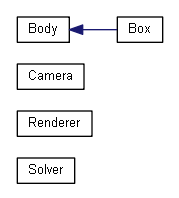
\includegraphics[width=0.3\textwidth]{figures/classes.png}
\caption{Diagram klas (opracowanie własne).}%
\label{rys:Podzial klas}
\end{figure}
Plik nagłówkowy \verb$stdafx.h$ zawiera informacje o wszystkich dołączonych do projektu plikach źródłowych, bibliotek oraz zdefiniowane stałe. Dzięki wykorzystaniu takiego rozwiązania możliwe jest łatwe zarządzanie projektem oraz zmniejszone jest ryzyko błędu wielokrotnego dołączania tej samej biblioteki lub pliku źródłowego.\\
Plik \verb$main.cpp$ zawiera inicjalizację instancji klas odpowiedzialnych za renderowanie oraz komunikację z układem GPU. Tworzone są tu również obiekty symulacji. Znajduje się tutaj również główna pętla aplikacji.\\
Klasa \verb$Camera$ zawiera implementację uproszczonej kamery, umożliwiającej poruszanie się po renderowanej scenie.
\verb$Renderer$ odpowiada za stworzenie okna aplikacji, ciągłe generowanie obrazu symulowanych brył, przemieszczanie kamery oraz przełączanie trybu pomiędzy wyswietlaniem brył oraz samych ich siatek.
Klasa \verb$Solver$ obejmuje komunikację z GPU oraz posiada implementację obliczeń fizycznych wykorzystujących CPU.
Klasa \verb$Renderer$, \verb$Solver$ oraz \verb$Camera$ zostały stworzone wykorzystując wzorzec projektowy Singleton\footnote{Singleton - kreacyjny wzorzec projektowy. Gwarantuje, że klasa będzie miała tylko jeden egzemplarz i zapewnia globalny dostęp do niego\cite{Wzorce projektowe}.}. Celem zastosowania wzorca jest ograniczenie liczby stworzonych instancji danej klasy do jednej oraz zapewnienie globalnego dostępu do stworzonego obiektu. W przypadku każdej klasy korzystającej z tego wzorca, implementacja sprowadza się do stworzenia statycznej metody zwracającej referencję do instancji obiektu. Wywoływana metoda dodatkowo tworzy obiekt klasy przy pierwszym jej uzyciu. Należy pamiętać, aby zarówno kontruktor jak i instancja klasy były składowymi prywatnymi, aby uniemożliwić stworzenie większej ilości obiektów danej klasy.\\
\verb$Body$ jest klasą bazową, zawierającą strukturę obiektu, metody ustawiające, pobierające oraz obliczające odpowiednie elementy struktury.
\verb$Box$ jest klasą dziedziczącą po klasie \verb$Body$. Ustawia ona typ tworzonej bryły oraz nadpisuje część metod obliczających z klasy bazowej.
Dodatkowo plik \verb$Phys.cl$ zawierający logikę obliczanych sił oraz przemieszczeń obiektów na~urządzeniu GPU.

\section{Struktury danych}
Ważnym elementem aplikacji jest struktura \verb$myBody$ zawarta w klasie \verb$Body$. Zawiera ona następujace dane:
\begin{itemize}
\item center -  centralny punkt obiektu w postaci trzech wartości typu zmiennoprzecinowego, odzwierciedlających położenie w globalnej przestrzeni trójwymiarowe,
\item lengths - długości odcinków od środka obiektu do jego krawędzi prowadzonych wzdłuż lokalnych osi układu współrzędnych,
\item velocity - aktualna wartość wektora prędkości,
\item angularVelocity - aktualna wartość wektora prędkości kątowej obiektu wyrażona w~postaci trzech liczb,
\item weight - masa bryły,
\item orientation - aktualny obrót obiektu wyrażony w postaci kwaternionu,
\item isActive - zmienna binarna określająca stan obiektu,
\item type - zmienna wskazująca na typ bryły,
\item points - obliczone współrzędne wierzchołków, służące do poprawnego wyrenderowania bryły.
\end{itemize}
Identyczna struktura znajduje się w pliku \verb$Phys.cl$. Położenie kolejnych elementów struktury zarówno w pliku kernela jak i pliku klasy musi być identyczne, gdyż w innym przypadku, np. zamieniając w strukturze kernela miejscami pola center oraz lengths, wartości używane od obliczeń byłyby zmienione i powodowałyby błędne wyniki.

\section{Przesyłanie danych między CPU a GPU}
Idea przesyłania danych pomiędzy pamięcią RAM a pamięcią urządzenia GPU została opisana w rozdziale siódmym. Po utworzeniu kontekstu oraz kolejki zadań, stworzony jest bufor o wielkości równej pamięci potrzebnej na przechowanie struktury dla jednej bryły pomnożonej przez liczbę brył biorących udział w symulacji. Dostęp do bufora jest typu CL\_MEM\_READ\_WRITE, co oznacza, iż możliwe jest zarówno odczytywanie jak i~zapisywanie do niego danych. Następnie uzupełniane są argumenty przesyłane do funkcji kernela:
\begin{itemize}
\item wkaźnik na bufor obiektów,
\item liczba obiektów biorących udział w symulacji,
\item czas, jaki upłynął pomiędzy kolejnymi iteracjami pętli.
\end{itemize}
Po wykonaniu operacji należy przekopiować z powrotem dane z bufora do listy obiektów. Umożliwienie zarówno odczytu jak i zapisu do jednego bufora pozwoliło zmniejszyć zapotrzebowanie na pamięć układu GPU. Aby jednak było to możliwe, operacje wykonywane na~danych znajdujących się w buforze musiały zostać zaimplementowane w taki sposób, by nie ingerować w elementy struktury wykorzystywane do sprawdzania kolizji z innymi bryłami. %implementacja aplikacji
\chapter{Wyniki}

Po stworzeniu aplikacji przeprowadzone zostały testy mające na celu sprawdzić wydajność aplikacji pod kątem czasu wykonania oraz porównanie wyników, wykonując te same obliczenia korzystając jedynie z mocy CPU. 
Poniżej zamieszczone zostały wyniki tych pomiarów.

\begin{figure}[h]
\centering
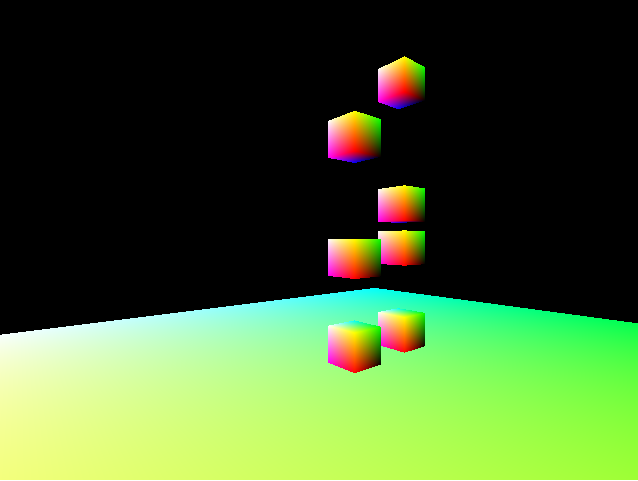
\includegraphics[width=0.4\textwidth]{figures/app1.png}
\caption{Przykładowy zrzut ekranu z aplikacji (opracowanie własne).}%
\label{rys:Przykladowy zrzut ekranu z aplikacji}
\end{figure}
\begin{figure}[h]
\centering
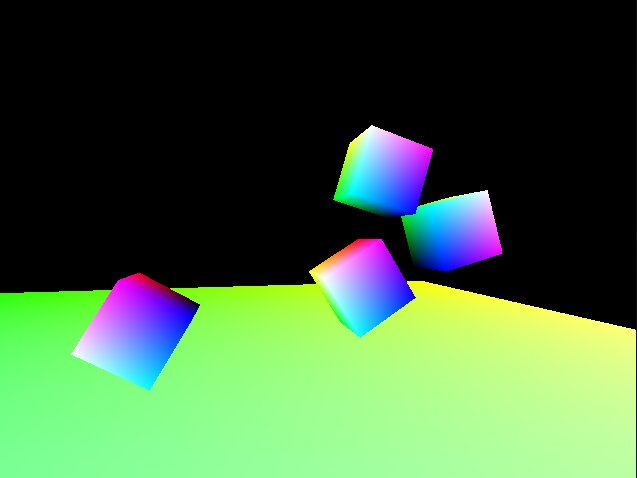
\includegraphics[width=0.4\textwidth]{figures/app2.png}
\caption{Zrzut ekranu z aplikacji po kolizji (opracowanie własne).}%
\label{rys:Zrzut ekranu z aplikacji po kolizji}
\end{figure}
\begin{figure}[h]
\centering
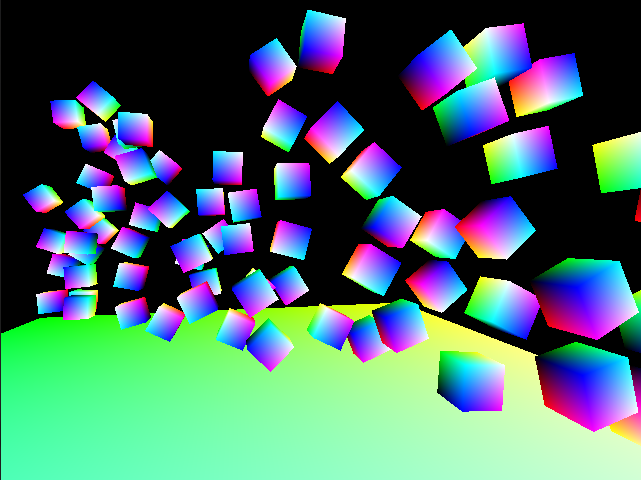
\includegraphics[width=0.5\textwidth]{figures/app3.png}
\caption{Zrzut ekranu z aplikacji po kolizji (opracowanie własne).}%
\label{rys:Zrzut ekranu z aplikacji po kolizji}
\end{figure}
\begin{tabular}{|c|c|c|}
\hline
Liczba brył & Czas wykonania GPU (ms) & Czas wykonania CPU(ms) \\
\hline
1 & 46.3 & 16.7\\
2 & 46.3 & 16.7\\
5 & 46.3 & 16.7\\
10 & 46.3 & 16.7\\
100 & 52.4 & 167.8\\
1000 & 90.6 & ponad 1000\\
\hline
\end{tabular}
\newline
\newline
\newline
Tabela przestawia uśrednioną wartość czasu potrzebną na wykonanie jednej iteracji zawierającej aktualizację pozycji obiektów oraz wyznaczanie kolizji i obliczanie wartości sił po zderzeniu. Każdy przedstawiony wynik to średnia arytmetyczna z 1000 pomiarów. Można zauważyć, iż czas potrzebny na wykonanie tych operacji w zakresie do 10 brył w symulacji jest niezmienny. Jednocześnie widać, że do tego momentu wykonywanie operacji na CPU przynosi większe korzyści, niż na GPU. Zdarzenie to spowodowane jest dodatkowym czasem potrzebnym na utworzenie buforów oraz przesyłanie ich do oraz z urządzenia GPU. Natomiast wraz ze wzrostem liczby symulowanych obiektów średni czas operacji zwięsza się zdecydowanie szybciej dla testu przeprowadzonego na CPU. Dzięki możliwości równoległego wykonywania operacji na wielu obiektach jednocześnie, czas potrzebny na wykonanie operacj rośnie zdecydowanie wolniej niż ma to miejsce przy wykorzystaniu CPU.\\ %wyniki
\chapter{Podsumowanie i wnioski}

W niniejszej pracy została pokazana symulacja bryły sztywnej z wykorzystaniem technologii OpenCL. Została również przedstawiona przenośność tego rozwiązania inne na plaftormy, takie jak procesory ogólnego zastosowania firmy Intel. Praca pokazuje również, że technologia OpenGL jest wystarczająca do wizualizacji przedstawionej symulacji. 
Dzięki wykorzystaniu mocy obliczeniowej karty Nvidia, wykorzystanie procesora CPU zostało odciążone. Dzięki możliwości równoległego przetwarzania instrukcji dla obiektów, wyniki obliczeń dla większej liczby obiektów były gotowe niemalże w tym samym czasie.\\
Niestety konieczność ciągłego przesyłania danych pomiędzy układem GPU a pamięcią RAM jest jednym z głównych powodów spowolnienia czasu wykonania całego cyklu obliczeń a co jest z tym związane, ograniczenie możliwości wykorzystania w pełni mocy układu. Nakład czasu potrzebny na przesłanie większej porcji danych został zredukowany dzięki ograniczeniu ilości tych danych, pozwalając, by część z nich została obliczona już po stronie GPU oraz poprzez brak konieczności tworzenia dodatkowej tablicy na obiekty biorące udział w~symulacji. \\
Wykorzystanie technologii OpenCL zapewnia przenośność oprogramowania, dzięki czemu umożliwia wykorzystanie zaproponowanego rozwiązania obliczeń fizycznych również na innych konfiguracjach wspierających odpowiednią wersję technologii. Dzięki temu możliwe jest przyspieszenie wykonania obliczeń korzystając nawet z budżetowych układów GPU dając zadawalające rezultaty.\\ %wnioski
\chapter*{Streszczenie angielskie}
\section*{Aim}
The purpose of this thesis is to create rigid body simulation using OpenCL framework to accelerate calculations, i.e. moving objects, finding collisions and responding to them. Moreover a simplified implementation of rendering using OpenGL will be created for~displaying the simulation.
\section*{Assumptions}
Thesis plan assumes usage of OpenCL at version 1.2 for boosting calculations, usage of~OpenGL at version 3.1 with additional library GLFW at version 3 for rendering. The base program will be written in C++.\\
Simulation will take place in a space with gravity set at 9.81$m \over s_2$ value and a substructure with mass close to infinity (m = $\infty$) that is unaffected by gravity.
\section*{Results and conclusions}
After implementation of application was completed, a series of test was run. The tests showed that although simulation was running faster on CPU with up to 10 bodies, using more object showed that GPU finished calculations for them faster than CPU. This is possible thanks to parallel processing many (if not all) calculations for rigid bodies. Another positive effect of using OpenCL is portability and possibility to move a computing solution to another hardware that supports the technology. With that aspect even bugdet GPU devices can be used and boost physical or mathematical calculations.
 %streszczenie eng
\begin{thebibliography}{999}

\bibitem{GamePhys} David M Bourg, \emph{Physics for Game Developers }, O'Reilly Media, November 2001
\bibitem{nVidia-1} 
gafferongames.com, \emph{Rotation and Inertia Tensors}, \texttt{http://gafferongames.com/virtualgo/}, witryna internetowa, stan na 01 września 2014
\bibitem{nVidia-1} 
gafferongames.com, \emph{OpenCL 1.2 Reference Pages}, \texttt{http://www.khronos.org/registry/cl/sdk/1.2/docs/man/xhtml/}, witryna internetowa, stan na 01 września 2014
\end{thebibliography}


\listoffigures

%\listoftables

%\newpage
%\thispagestyle{empty}
%\begin{textblock}{1}(-2.65,-1.65)
%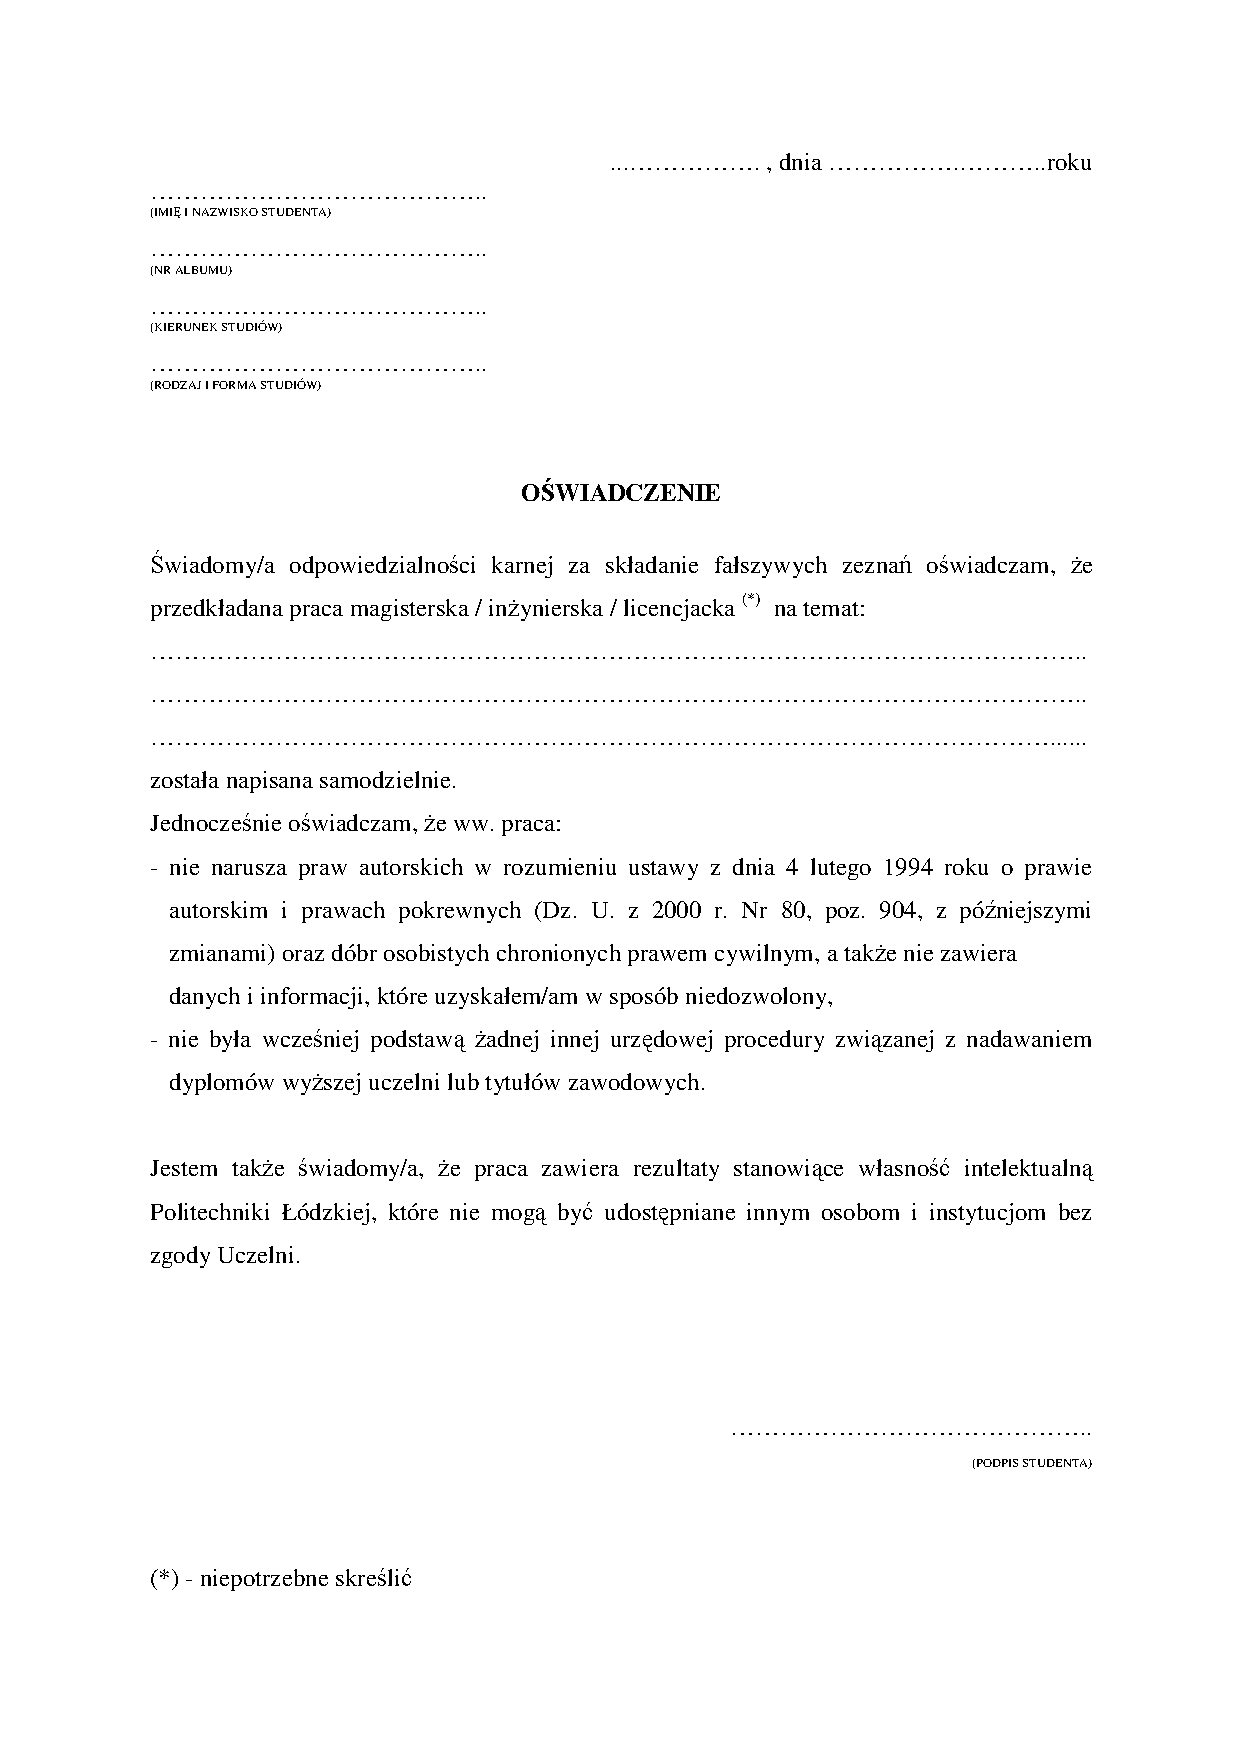
\includegraphics{figures/oswiadczenie_o_samodzielnosci.pdf}
%\end{textblock}
%\newpage
%\thispagestyle{empty}
%\begin{textblock}{1}(-2.65,-1.65)
%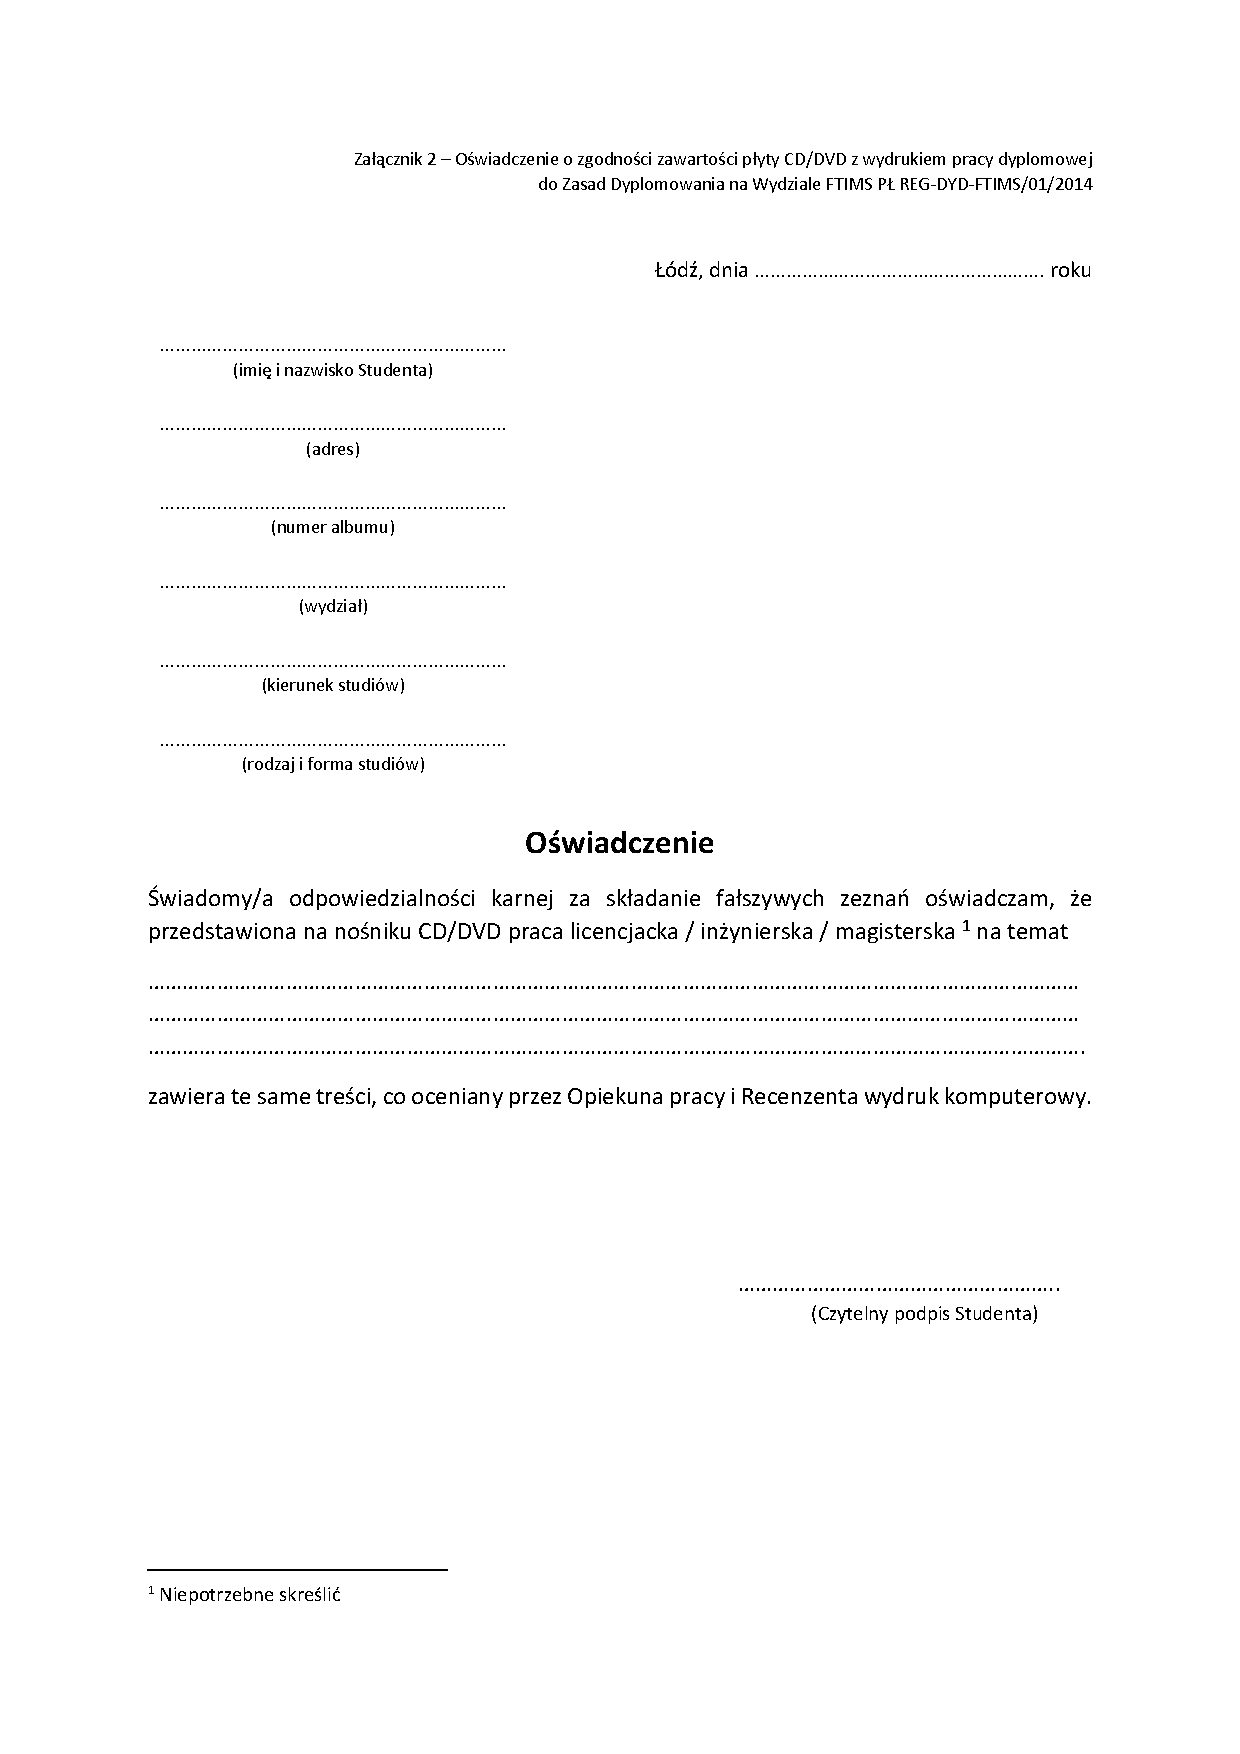
\includegraphics{figures/Zalacznik2.pdf}
%\end{textblock}
\end{document}
